\clearpage
\section{Model specifics}
\label{sec:setup}
The version of ROMS we use is downloaded from the main ROMS repository\footnote{\texttt{http://www.myroms.org/svn/src/trunk}}, which includes the latest version from Hernan Arango (the Rutgers branch). This version is without sea ice, but in contrast to most other ROMS versions allows data assimilation.

ROMS consists of several built-in schemes and algorithms, and it uses C-preprocessing to activate the various physical and numerical options. ROMS is a very modern and modular code written in F90/F95. The entire input and output data structure of the model is via NetCDF which facilitates the interchange of data between computers, user community, and other independent analysis software.
%%%%%%%%%%%%%%%%%%% Figure 2 Bathymetry and currents in the Drøbak area %%%%%%%%%%%%%%%
\begin{figure}[t]
  \begin{pspicture}(0,0)(15.5,10)
% Include graphs
   \rput[b](6.5,0){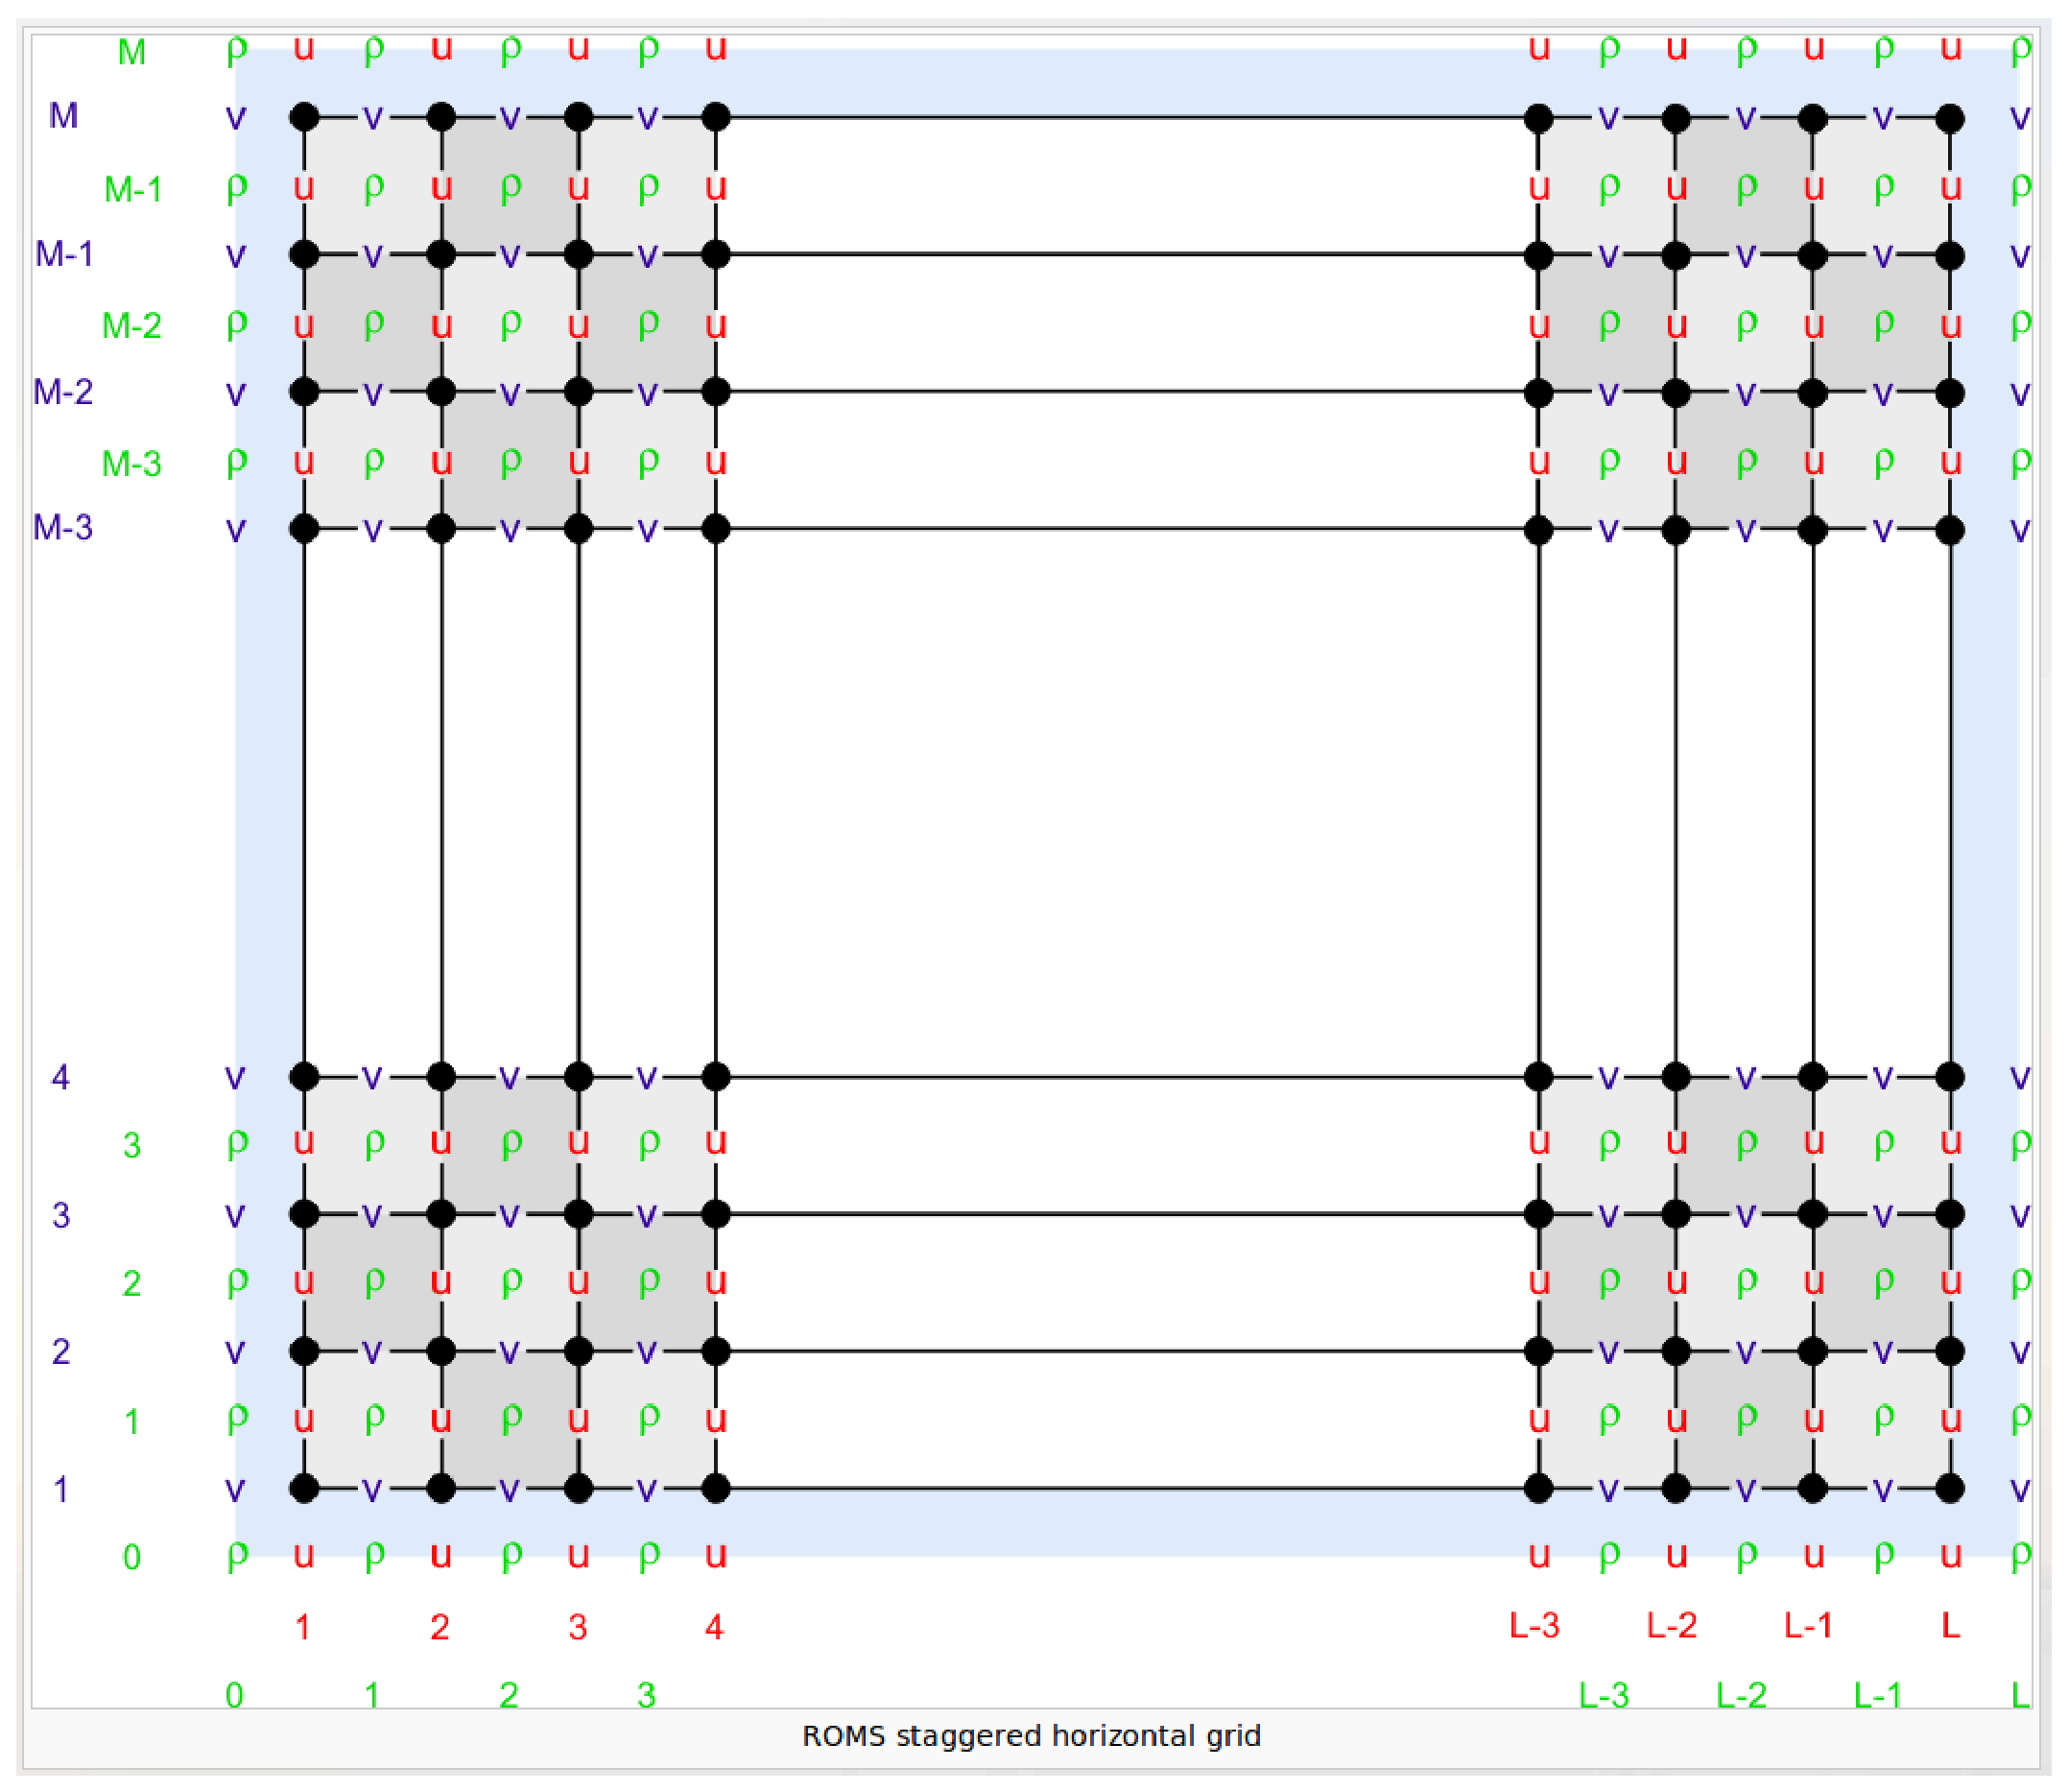
\includegraphics[height=10cm]{ROMS_staggered_horizontal_grid}}
   \rput[rt](15.5,10){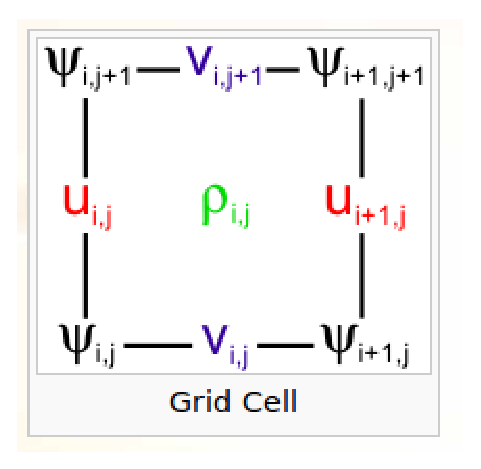
\includegraphics[height=3cm]{ROMS_grid_cell_numbering}}
  \end{pspicture}
  \caption{\small The horizontal distribution and numbering system of variables in the ROMS grid. The figure is downloaded from the \texttt{http:www.myroms.org} website.}
  \label{fig:romsgridh}
\end{figure}



In the horizontal the model state variables are staggered using an Arakawa C-grid as shown by Figure \ref{fig:romsgridh}. The free-surface, density, and active/passive tracers are located at the center of the cell ($\rho$ points) whereas the horizontal current components ($u$, $v$) are located at the west/east and south/north edges of the cell, respectively. In ROMS all the arrays containing state variables are dimensioned with the same size in the horizontal to facilitate parallelization. The size of the model's horizontal grid is defined in the ROMS input file (\texttt{ocean.in}) with interior points only (denoted $L-1$ and $M-1$ in Figure \ref{fig:romsgridh}). However, all input forcing files must, and output result files do, contain fields at the full grid, which includes the one extra grid point in the boundary zone.

In the vertical ROMS make use of a stretched terrain-following coordinate denoted $s=s(x,y,z,t)$, sometimes referred to as modified $\sigma$-coordinates \citep{song:haidv:1994}. As a result, each grid cell has a different level thickness (denoted $H_z = \pzs z$) and volume. The model state variables are vertically staggered so that horizontal momentum, density, and active/passive tracers are located at the center of the grid cell. The vertical velocity and vertical mixing variables ($Akt$, $Akv$, etc) are located at the bottom and top faces of the cell as displayed by Figure \ref{fig:romsgridv}. The stretched coordinate allows increased resolution in areas of interest, such as thermocline and bottom boundary layers. 
%%%%%%%%%%%%%%%%%%% Figure 2 Bathymetry and currents in the Drøbak area %%%%%%%%%%%%%%%
\begin{figure}[t]
  \begin{pspicture}(0,0)(15,10)
% Include graphs
   \rput[b](7.5,0){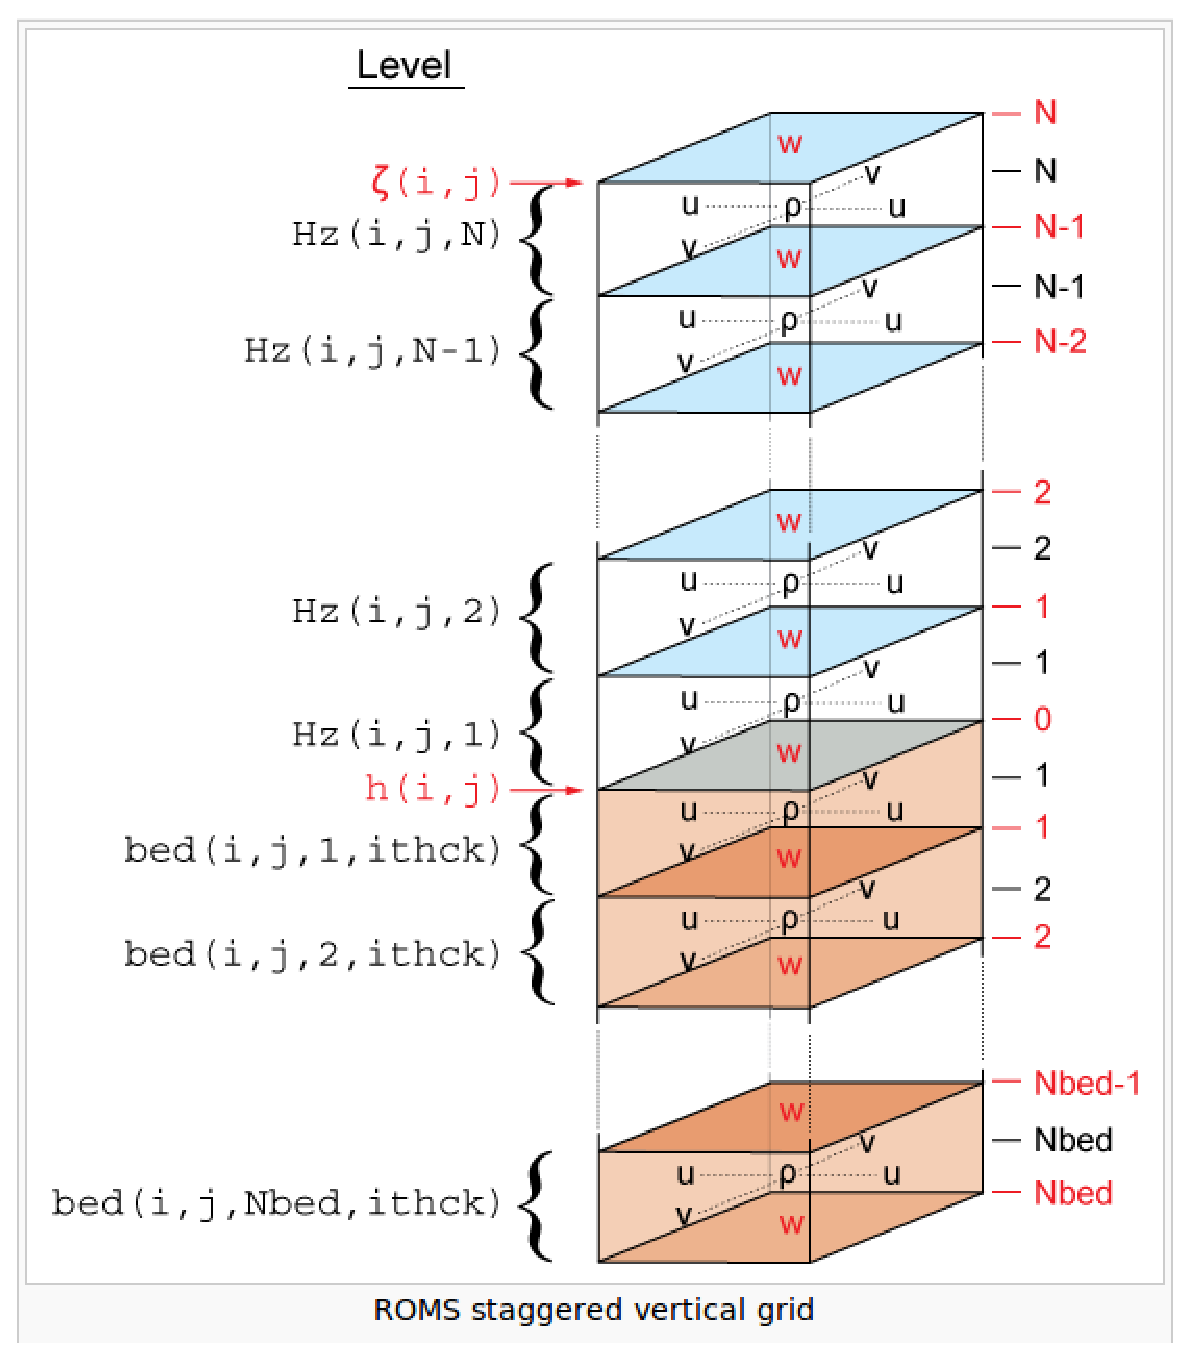
\includegraphics[height=10cm]{ROMS_staggered_vertical_grid}}
  \end{pspicture}
  \caption{\small The vertical distribution and numbering system of variables in the ROMS grid. The figure is downloaded from the \texttt{http:www.myroms.org} website.}
  \label{fig:romsgridv}
\end{figure}



Regarding the FjordOs CL model we opted for 42 $s$-layers with an increased resolution in the surface layer and a reduced resolution near the bottom. This was achieved by letting $Vtransform=2$, $Vstretching=2$, $h_c = 100$ m, $\th_s = 6.0$ and $\th_b = 0.1$, where $h_c$ is a critical depth above which the vertical spacing of the $s$-levels become nearly uniform and independent of the local depth $h$ as long as $h >> h_c$. The minimum depth was set to $h_min=10$ m. By having the $s$-levels more confined to the surface layers less smoothing is necessary to minimize the pressure gradient error inherent in all terrain-following coordinate models \citep{haney:1991}. The smoothing is controlled by two parameters referred to as the $r$-factors (see Section \ref{subsec:bathy}). An example of the vertical distribution of the $s$-levels is shown by Figure \ref{fig:roms_slevels}.
%%%%%%%%%%%%%%%%%%% Figure 2 Bathymetry and currents in the Drøbak area %%%%%%%%%%%%%%%
\begin{figure}[t]
  \begin{pspicture}(0,0)(15,10)
% Include graphs
   \rput[b](7.5,0){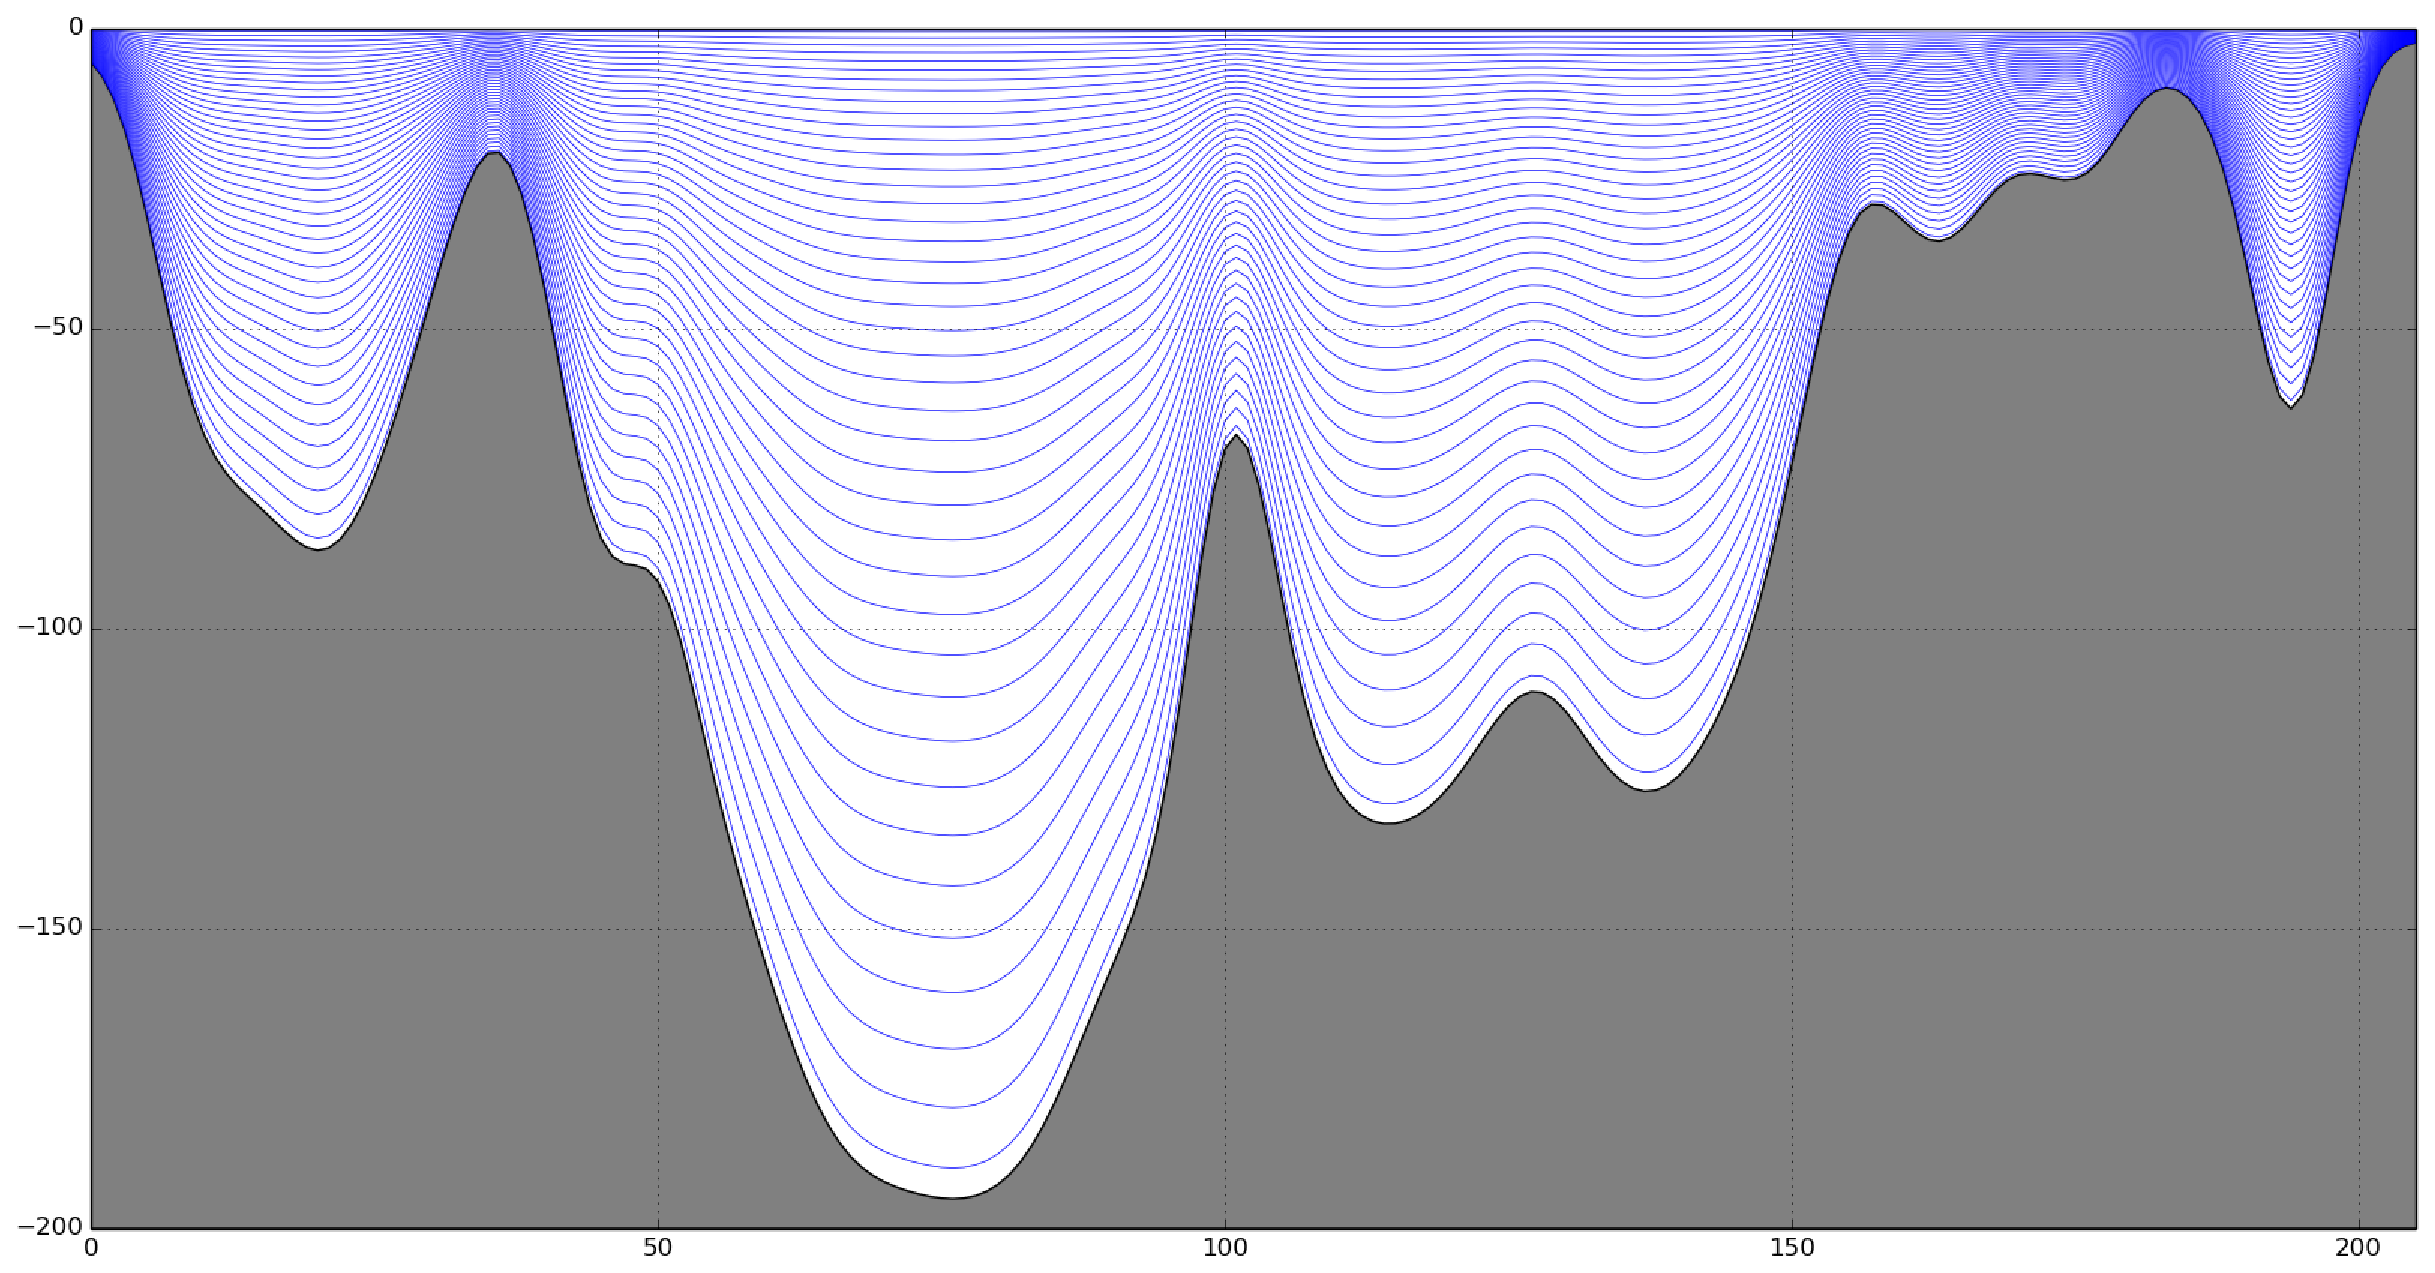
\includegraphics[height=5cm]{fjordos_vertical_coordinates}}
  \end{pspicture}
  \caption{\small Sketch of the vertical distribution of $s$-levels in the FjordOs model (cross-section at Breiangen, y=600).}
  \label{fig:roms_slevels}
\end{figure}



ROMS has several options that determines the numerical schemes for lateral advection of momentum and tracers. In the results displayed in Section \ref{sec:resul} we have employed a fourth-order, centered advection scheme. This necessitate the application of explicit lateral eddy viscosity and diffusion. To parametrize the subgrid-scale vertical mixing processes we use the Generic Length Scale (GLS) scheme  \citep{umlau:burch:2003}. Values chosen for the various parameters and options activated to derive the results exhibited by Section \ref{sec:resul} are listed in Table \ref{tab:parameters}. 

To run the model several external inputs or forcing have to be supplied, such as atmospheric input, river input, tides, and input of sea level, currents and hydrography at the model's open lateral boundaries, in addition to bathymetry as described in Section \ref{sec:forcing}.   
\begin{table}[h]
 \begin{center}
  \caption{List of FjordOs CL model set-up parameters.}
   \begin{tabular}{lccl}
   \hline
    Parameter				& Symbol	& Value	& Unit		\\
   \hline
    Vtransform				& -		& 2 	& -		\\
    Vstretching 			& -		& 4	& -		\\
    Number of layers			& $k$ 		& 42 \\
    %Explicit lateral eddy viscosity	& $A_M$		& 	& m$^2$s$^{-2}$	\\
    Critical depth			& $h_c$		& 50	& m		\\
    Surface resolution factor		& $\th_s$	& 3.0	& -		\\
    Bottom resolution factor		& $\th_b$	& 0.5	& -		\\
    %.. 					& ..		& ..	&		\\
   \hline
   \end{tabular}
  \label{tab:parameters}
 \end{center}
\end{table} 



%%%%%%%%%%%%%%%%%%%%%%%%%%%%%%%%%%%%%%%%%%%%%%%%%%%%%%%%%%%%%%
\section{Bathymetry and external forcing}
\label{sec:forcing}
% % % % % % % % % % % % % % % % % % % % % % % % % % % % % % % % 
\subsection{Bathymetry}
\label{subsec:bathy}
The bathymetry data for the FjordOs CL model were collected from ?????? and the Hydrographic service (Statens Kartverk Sj{\o}). The original resolution was 50 m. Modifications of some of the topographical features were needed to fulfill the restriction of avoiding one-point bays in ROMS. Additionally, effort was made in opening up narrow straits important for the local circulation, in particular advection of brackish water originating from rivers. To avoid model instability and/or spurious deep currents the final masked bathymetry is smoothed to fulfill a requirement on the ROMS slope or $r_{x1}$-factor \citep{beckm:haidv:1993}, defined as
\be
 r_{x1} = \frac{ h_{i-1} - h_{i} }{ h_{i-1} + h_{i} }
\ee
where $h$ is the bottom depth and the index $i$ indicates a model grid point. The final bathymetry in FjordOs CL has a maximum $r_{x1} = ?????$.

In addition, Haney (1991) argues that in order for difference schemes to be hydrostatically
consistent, the parameter settings must be defined so that
\be
\label{eq:haney}
 \left| \frac{s}{h} \px h\right|\frac{\Dx}{\Ds} < 1
\ee
where $s$ denotes the value of the terrain-following $s$-layer (0 at the surface, -1 at the bottom), $\px h$ is the difference in depth over a grid cell, $\Dx$ is the grid size and $\Ds$ is the vertical distance between $s$-layers. For instance in a grid cell with total depth of $h_i=1000$ m, with a neighboring depth of $h_i-1=900$ m, with a grid resolution $\Dx=800$ m, near the seabed between $s$-layer 0.9 and 1.0, the Haney number would be 1. In practice the Haney number is estimated by
\be
 r_{x2} = r_{x1}\frac{Z_w(i,j,k) - Z_w(i-1,j,k) + Z_w(i,j,k-1) - Z_w(i-1,j,k-1)}
                     {Z_w(i,j,k) + Z_w(i-1,j,k) - Z_w(i,j,k-1) + Z_w(i-1,j,k-1)}
\ee
where $Z_w$ is the depth of the water column at grid coordinates ($i,j$) and at $s$ level $k$. In the case where the second deepest $s$-level of grid cell ($i,j$) has equal depth to the deepest level in grid cell ($i-1,j$) the Haney number will be 1. Obeying the criteria (\ref{eq:haney}) ensures that for a certain grid size the vertical grid increment is small enough for the $s$-layer immediately above (below) remains above (below) within the distance of one grid interval. Although there is no mathematically well-defined thresholds a rule of thumb is $r_{x2} \lesssim 10$. There is no consensus in the ROMS community on the upper limit for $r_{x2}$ though. Thus one has to consider the recommendations on thresholds to be the outcome of practical experience. For instance Kate Hedstr{\o}m allows a Haney number of several tens while Alexander Shchepetkin considers a value below 3 as ``safe and conservative'' and values above 8-10 as ``insane''\footnote{ROMS Discussion Forum (\texttt{https://www.myroms.org/forum/viewtopic.php?f=14\&t=612)}}. It boils down to controlling the pressure gradient error. Recent examples for Norwegian waters and fjords are \cite{albre:etal:2011} and \cite{staal:roed:2016}. The latter applied ROMS for the inner part of the Oslofjord inside of the {\DR} sill. 

% % % % % % % % % % % % % % % % % % % % % % % % % % % % % % % % 
\subsection{Atmospheric forcing}
\label{subsec:atmos}
The necessary atmospheric input is extracted from the AROME-MetCoOp model that runs operationally at MET Norway \citep{mulle:etal:2015}. It is a convective scale (non-hydrostatic) model providing forecasts with a lead time of 66 hours four times a day from analyses at 00, 06, 12 and 18 UTC. It has a grid resolution of 2.5 km, and was made operational in March 2014. Available to us are analyses and forecasts saved every four hours since April 2014, as well as real time forecasts covering the are shown in Figure \ref{fig:arome}.
%%%%%%%%%%%%%%%%%%%%%%%%%%% Figure 3 Godafoss %%%%%%%%%%%%%%%%%%%%%%%%%%%%%%%
\begin{figure}[t]
 \begin{center}
  \begin{pspicture}(0,0)(15,10)
% Include graphs
   \rput[b](7.7, 0.0){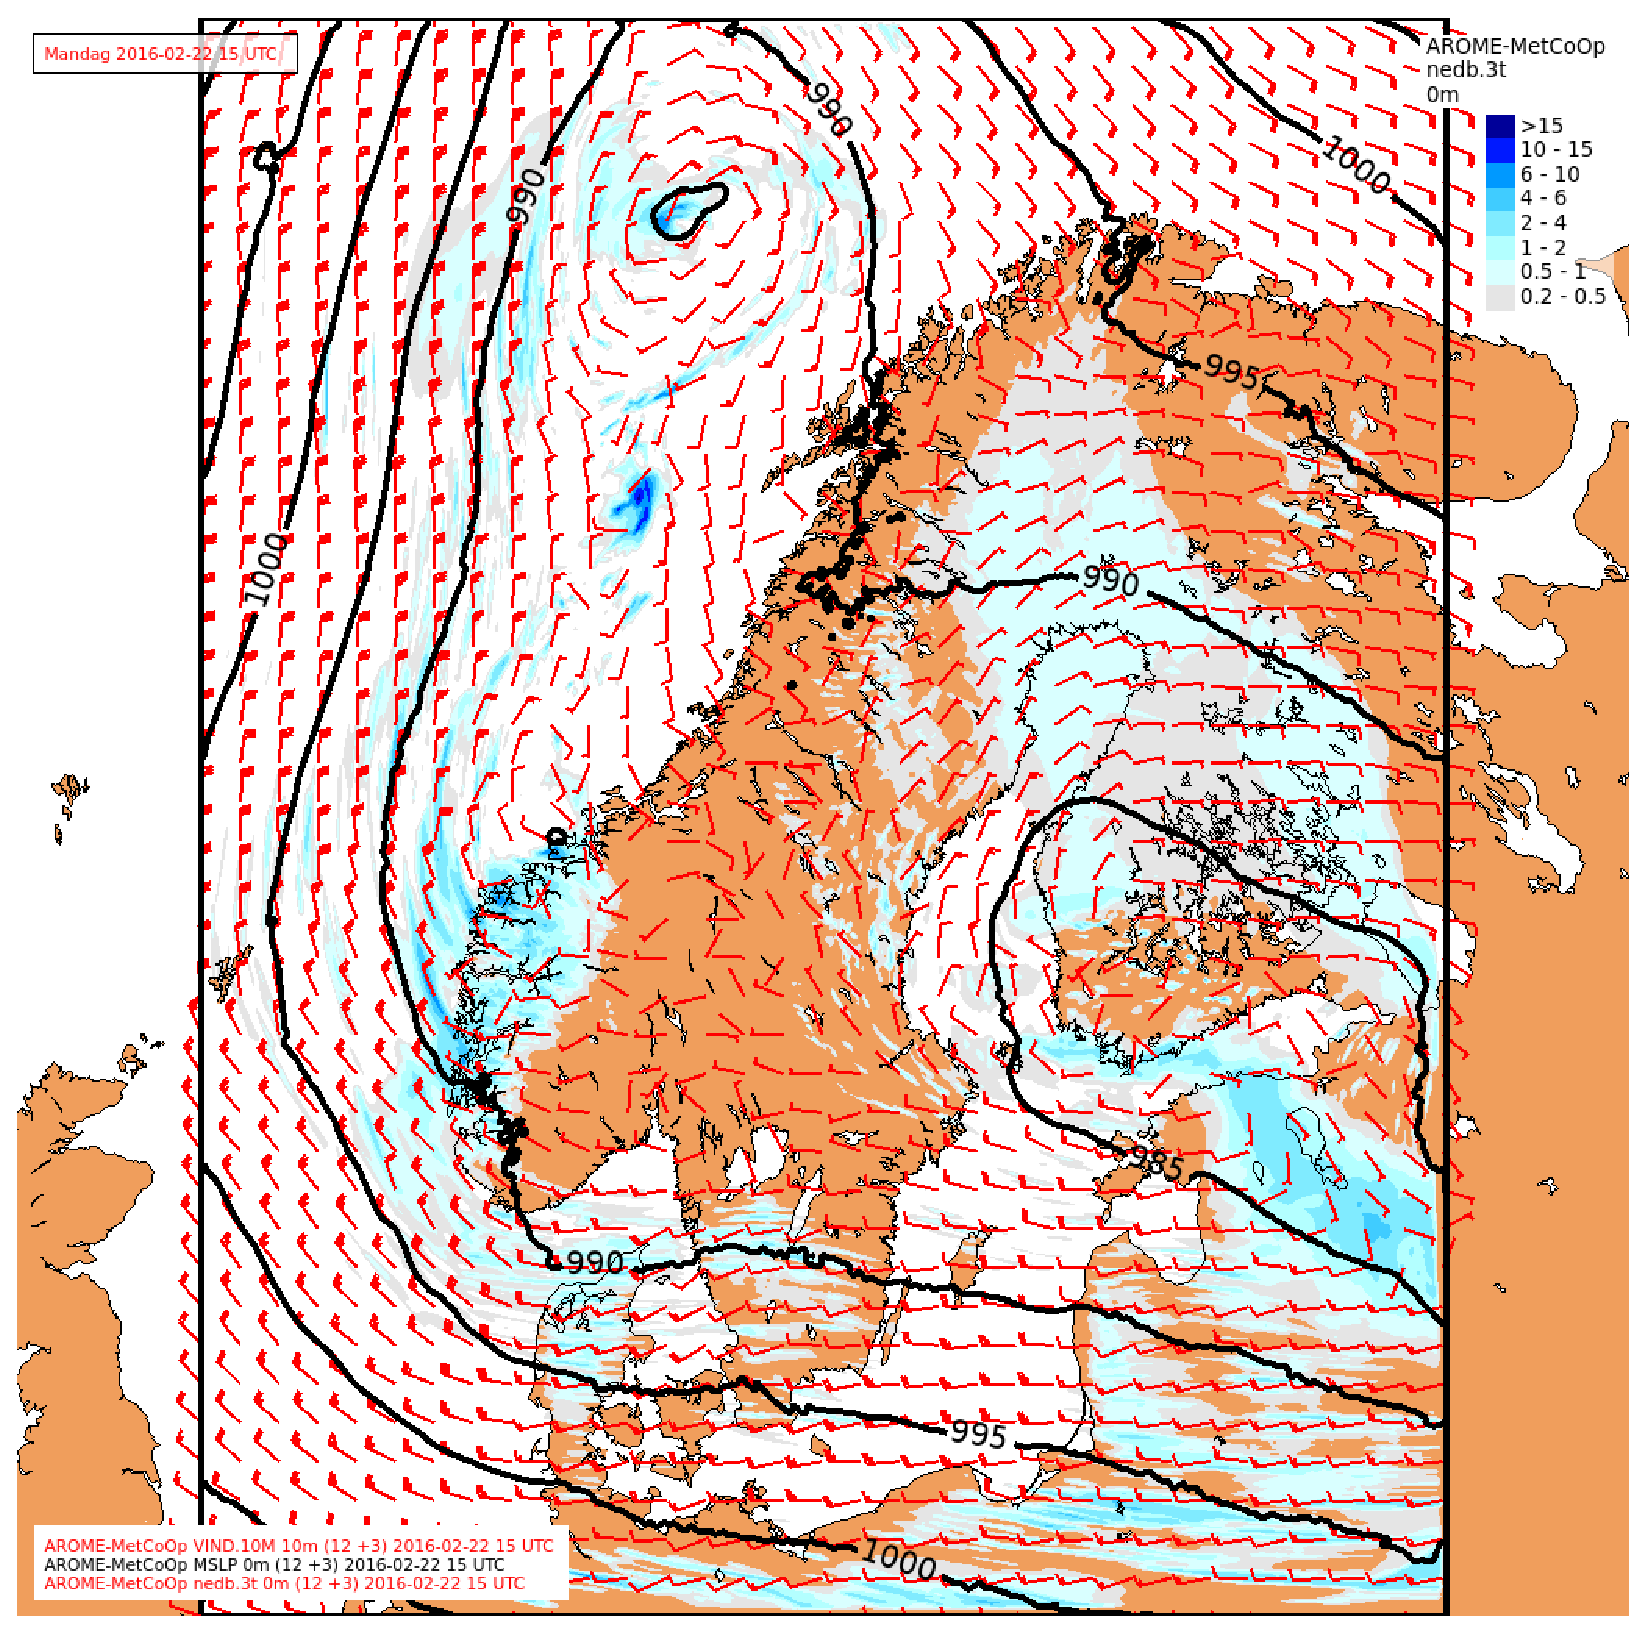
\includegraphics[height=10cm]{AROME_2016-02-22_15UTC}}
  \end{pspicture}
  \caption{\small The area covered by the Arome-MetCoop model. Shown is the forecasted (lead time 3 hrs) mean sea level pressure in hPa (black solid lines, countour interval = 5 hPa), 3 hourly precipitation, and 10 m wind valid at 1500UTC on February 22, 2016. Color bar indicates precipitation with a variable contour interval in the range 0.2-15 mm or larger (deep blue).} 
  \label{fig:arome}
 \end{center}
\end{figure}



We extract from AROME-MetCoOp, as listed in Table \ref{tab:atmos_para}, surface analysis and forecasts of wind, pressure, temperature, and cloud cover daily at 00, 06, 12, 18 UTC. We also extract model level analysis of humidity at the same frequency. In addition are extracted surface forecast of precipitation and long wave radiation as 12 hrs accumulated fields at 00 and 12 UTC, and short wave radiation as 24 hrs accumulated fields at 00 and 12 UTC. AROME-MetCoOp store all these parameters at its grid resolution. From these parameters and variables fluxes are computed using the internal bulk-flux routines in ROMS \citep[e.g.,][]{roed:deber:2004}. FjordOs CL also computes internally, from analytic expressions, net long wave radiation and short wave radiation.
\begin{table}[t]
 \begin{center}
  \caption{List of atmospheric forcing parameters.}
   \begin{tabular}{lccl}
   \hline
    					& ROMS			& 		\\
    Parameter name			& input name		& Unit		\\
   \hline
    10 m U wind component		& Uwind			& ms$^{-1}$	\\
    10 m V wind component 		& Vwind			& ms$^{-1}$	\\
    2 m air temperature			& T$_{air}$		& $^{\text{o}}$C	\\
    Mean sea level pressure		& P$_{air}$		& hPa		\\
    Total cloud cover			& cloud			& -		\\
    Specific humidity			& Q$_{air}$		& g kg$^{-1}$	\\
    Total precipitation			& rain			& kgm$^{-2}$s$^{-1}$		\\
   \hline
   \end{tabular}
  \label{tab:atmos_para}
 \end{center}
\end{table} 



% % % % % % % % % % % % % % % % % % % % % % % % % % % % % % % % 
\subsection{Input at open lateral boundaries}
\label{subsec:lateral}

%    %    %    %    %    %    %    %    %    %    %    %    %   
\subsubsection{De-tided input}
\label{subsubsec:detid}
The FjordOs CL grid has one wide open boundary located at its southern end towards the Skagerrak. Here we use input from the NorKyst800 model in the form of daily mean (de-tided) values of sea level, currents and hydrography. The NorKyst800 model covers the Norwegian coast including the Skagerrak and the Oslofjord with a grid resolution of 800 m as shown by Figure \ref{fig:n800}. To include the forcing from the NorKyst800 model a one-way nesting technique is employed as described in \cite{march:etal:2001}.  

The NorKyst800 is run operationally at MET Norway once a day and provides hourly forecasts with a lead time of 66 hrs. Daily mean values are computed and stored as netCDF files. These fields with some modifications may in addition be used as initial values to "cold" start FjordOs (Section \ref{sec:resul}). The archive containing daily mean values is updated automatically and adds back to 2012. The hourly forecast values are stored and archived one week back in time only. Both archives are available from MET Norway's thredds server\footnote{\texttt{http://thredds.met.no/thredds/fou-hi/norkyst800m.html}}. As input at the lateral open boundary FjordOs CL requires daily mean sea level values in addition to daily mean depth profiles of currents temperature and salinity.

%    %    %    %    %    %    %    %    %    %    %    %    %   
\clearpage
\subsubsection{Tidal forcing}
\label{subsubsec:tides}
The daily mean values extracted from NorKyst800 are viewed as being crudely de-tided. To get tides into the FjordOs CL model, tidal elevation and tidal (barotropic) currents have to be specified separately and superimposed on the daily mean NorKyst800 input. 
%%%%%%%%%%%%%%%%%%%%%%%%%%% Tidal componetns %%%%%%%%%%%%%%%%%%%%%%%%%%%%%%%%%%%%%%
%\clearpage
\begin{table}[t]
 \caption{Simulated tidal amplitudes [cm] and phases [deg] for a location close to the Viker tidal gauge station. The column "ATPXO" refers to the simulated tides using the TPXO Atlantic data base as input, while the column "Modified" refers to a run using adjusted tides as input. The column "Observed" refers to the observed tides at the nearby Viker tidal gauge station and is added for comparison.}
 \label{tab:1}
 \centering
 \newcolumntype{+}{D{+}{\pm}{2}}
% \begin{tabular}{|c|r|++|++|++|} 
 \begin{tabular}{cr++++++} 
  \hline
  Con-    & \mc{1}{c}{Period}      & \mc{2}{c}{Observed}       & \mc{2}{c}{ATPXO}           & \mc{2}{c}{Modified}\\
  stit.   & \mc{1}{c}{[hrs]} 
                    & \mc{1}{c}{[cm]} 
                                   & \mc{1}{c}{[deg]} 
                                                & \mc{1}{c}{[cm]} 
                                                               & \mc{1}{c}{[deg]} 
                                                                             & \mc{1}{c}{[cm]} 
                                                                                            & \mc{1}{c}{[deg]}\\
  \hline
  M$_2$  & 12.4206 & 12.4+0.7 & 115+3  &  9.7+1.1 & 122+6   & 11.8+0.3 & 105+1  \\
  N$_2$  & 12.6583 &  2.8+0.7 &  69+14 &  5.7+1.1 &  81+11  &  3.1+0.3 &  69+5  \\
  S$_2$  & 12.0000 &  2.3+0.7 &  48+15 &  5.1+1.0 &  81+11  &  3.2+0.3 &  67+5  \\
  O$_1$  & 25.8193 &  2.1+0.7 & 282+20 &  3.7+0.4 &  19+8   &  2.9+0.2 & 338+3  \\
  M$_4$  &  6.2103 &  1.4+0.2 & 287+7  &  0.7+0.2 &  25+17  &  1.1+0.0 & 354+1  \\
  Q$_1$  & 26.8684 &  1.0+0.6 & 221+42 &  0.1+0.3 & 215+154 &  0.1+0.1 & 253+156\\
  K$_1$  & 23.9345 &  0.7+0.6 &  98+49 &  1.2+0.5 & 212+23  &  0.1+0.1 & 198+97 \\
  MN$_4$ &  6.2692 &  0.4+0.2 & 270+24 &  1.0+0.2 & 141+12  &  0.3+0.0 &   7+3  \\
  MS$_4$ &  6.1033 &  0.4+0.2 &   5+28 &  1.1+0.2 & 111+12  &  0.6+0.0 &  80+1  \\
   \hline
 \end{tabular}
\end{table}




The tidal input in terms of tidal elevations and currents are based on the TPXO Atlantic database \citep[][hereafter ATPXO]{egber:erofe:2002}\footnote{\texttt{http://volkov.oce.orst.edu/tides/AO.html}}. Before supplying them to the FjordOs CL model they were first modified using measured tides at the Viker tidal gauge station located close to the southern boundary in the Hvaler Archipelago. Included are the nine tidal constituents listed in Tables \ref{tab:1} and \ref{tab:2}. As is evident semi-diurnal constituent M$_2$ is by far the most dominant one, but also N$_2$ and S$_2$ contributes. 
\begin{table}[t]
%\vspace{-1.5cm}
  \caption{As Table \ref{tab:1}, but for the Oscarsborg tidal gauge station.}
  \label{tab:2}
  \centering
 \newcolumntype{+}{D{+}{\pm}{2}}
 \begin{tabular}{cr++++++} 
  \hline
  Con-    & \mc{1}{c}{Period}      & \mc{2}{c}{Observed}       & \mc{2}{c}{ATPXO}           & \mc{2}{c}{Modified}\\
  stit.   & \mc{1}{c}{[hrs]} 
                    & \mc{1}{c}{[cm]} 
                                   & \mc{1}{c}{[deg]} 
                                                & \mc{1}{c}{[cm]} 
                                                               & \mc{1}{c}{[deg]} 
                                                                             & \mc{1}{c}{[cm]} 
                                                                                            & \mc{1}{c}{[deg]}\\
  \hline
  M$_2$   & 12.4206 & 14.1+0.7 & 132+3  & 11.1+1.2 & 128+7   & 13.7+0.3 & 111+2      \\
  N$_2$   & 12.6583 &  3.0+0.8 &  85+15 &  6.6+1.4 &  86+10  &  3.6+0.4 &  75+6      \\
  S$_2 $  & 12.0000 &  2.7+0.8 &  70+18 &  6.1+1.3 &  85+11  &  3.7+0.4 &  70+7      \\
  O$_1$   & 25.8193 &  2.1+0.7 & 286+17 &  3.9+0.5 &  21+8   &  3.1+0.2 & 340+4      \\
  M$_4$   &  6.2103 &  2.1+0.3 & 332+8  &  1.4+0.4 &  44+19  &  2.0+0.0 &  14+1      \\
  Q$_1$   & 26.8684 &  1.0+0.7 & 230+36 &  0.2+0.4 & 204+126 &  0.0+0.2 & 190+165    \\
  K$_1$   & 23.9345 &  1.2+0.5 & 101+35 &  1.1+0.5 & 213+27  &  0.1+0.2 &  44+79     \\
  MN$_4$  &  6.2692 &  0.6+0.3 & 316+26 &  2.0+0.4 & 163+14  &  0.5+0.0 &  29+3      \\
  MS$_4$  &  6.1033 &  0.5+0.3 &  57+32 &  2.2+0.4 & 135+11  &  1.3+0.0 & 106+1      \\
  \hline
 \end{tabular}
\end{table}





The rationale for the modification of the tidal input is that the resolution of the ATPXO, which is 1/30$^{\textrm{o}}$, is too coarse to get the exact phase and amplitude of the tides in Skagerrak correct. To modify the tides we first imposed the nine constituents on the open boundary of tides from the ATPXO database, and let it run for more than a year (the actual period was 12:00 UTC, April 1, 2014 - 12:00 UTC, September 28, 2014). Time series of water level from a location near the Viker and Oscarsborg tidal gauge stations were then extracted and analyzed based on the T\_Tide package described by \cite{pavlo:etal:2002}. The results are shown under column ``ATPXO'' in Tables \ref{tab:1} and \ref{tab:2}. For comparison we have also extracted and analyzed the observed time series from the Viker and Oscarsborg tidal gauge stations compiled from the Norwegian Coastal Administration (Tidevannstabeller for den norske kyst med Svalbard, 2008). The result of this analysis is shown in column ``Observed'', and clearly show that the simulated tides off the mark.  

To better match the observations tidal amplitudes and corresponding phases at the Viker tidal gauge station were then modified by computing an amplitude factor, $c^{(n)}$, and a phaseshift, $\Delta\phi^{(n)}$ for each tidal component $n$ according to:
\beq
  c^{(n)} &=& a^{(n)}_{obs} / a^{(n)}_{sim} \\
  \Delta \phi^{(n)} &=& \phi^{(n)}_{obs} - \phi^{(n)}_{sim}
\eeq
where $a^{(n)}$ is the amplitude and $\phi^{(n)}$ is the phase for tidal component number $n$ of the water level in the column ``ATPXO''. New amplitudes and phases at the boundary were then calculated using the computed amplification factor and phaseshift on both water level and velocity. The modified tides were then supplied to the FjordOs CL and run for a year with tidal forcing only. The new results were then analyzed exactly as for the ATPXO run. The resulting new tidal amplitudes and periods for the locations close to the Viker and Oscarsborg tidal gauge stations are shown in Tables \ref{tab:1} and \ref{tab:2} in column ``Modified''. The results are clearly improved at both stations. In particular we are pleased with the results close to the Oscarsborg tidal gauge station which may be viewed as a control station in that it is far away from the southern boundary where the tidal forcing is imposed.  


%  %  %  %  %  %  %  %  %  %  %  %  %  %  %  %  %  %  %  %  %  

\subsection{River input}
\label{subsec:river}
The influence of the freshwater discharged to the Oslofjord by way of the many rivers surrounding it is well known. A relevant example is shown by Figure \ref{fig:salt_hele} constructed from a test run with an earlier version of the FjordOs CL model. In particular the impact on the daily mean sea surface salinity of Norway's two largest rivers, namely Glomma to the southeast and Drammenselva to the northwest, is evident. As shown it tends to create salinity fronts that in turn give rise to high lateral as well as vertical shear currents. From time to time these fronts are even strong enough to generate instabilities. To obtain a realistic, high resolution picture of the circulation in the Oslofjord it is therefore paramount to include the input from these and other smaller rivers.
% %%%%%%%%%%%%%%%%%%%%%%%%%% Figure 1 Oversiktskart %%%%%%%%%%%%%%%%%%%%%%%%%%%%
\begin{figure}[t]
 \setlength{\unitlength}{1.0cm}
 \begin{center}
  \begin{pspicture}(0,0)(15,9)
% Include graphs
   \rput[bl](0,0){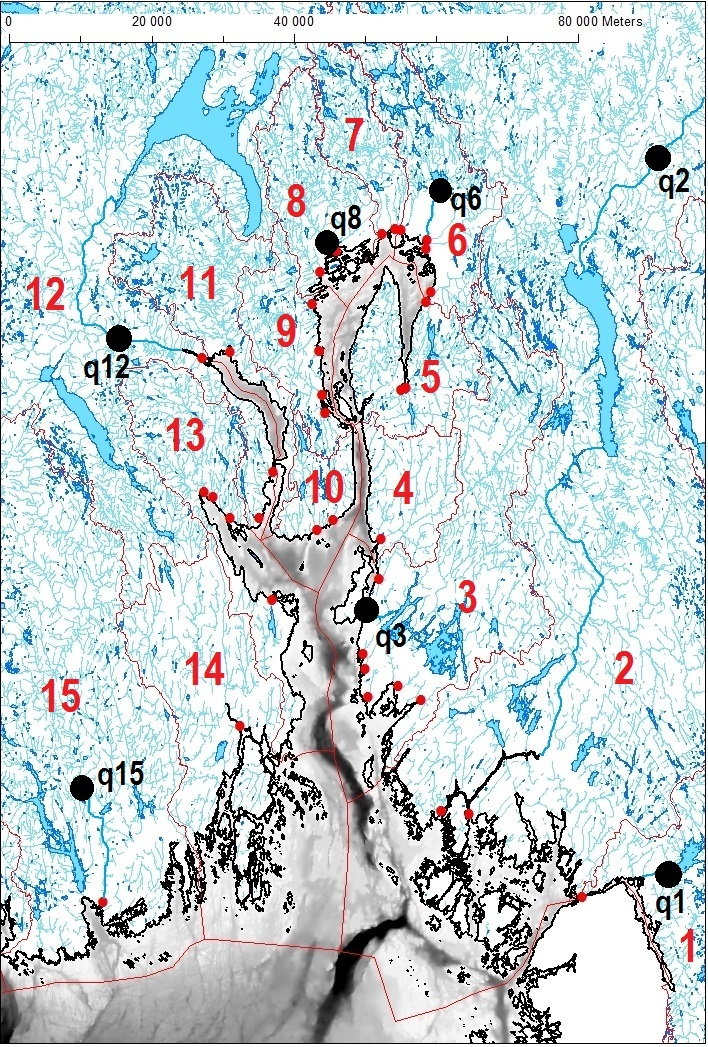
\includegraphics[height=9cm]{Elver_Oslofjorden_v4}}
   \rput[br](15,0){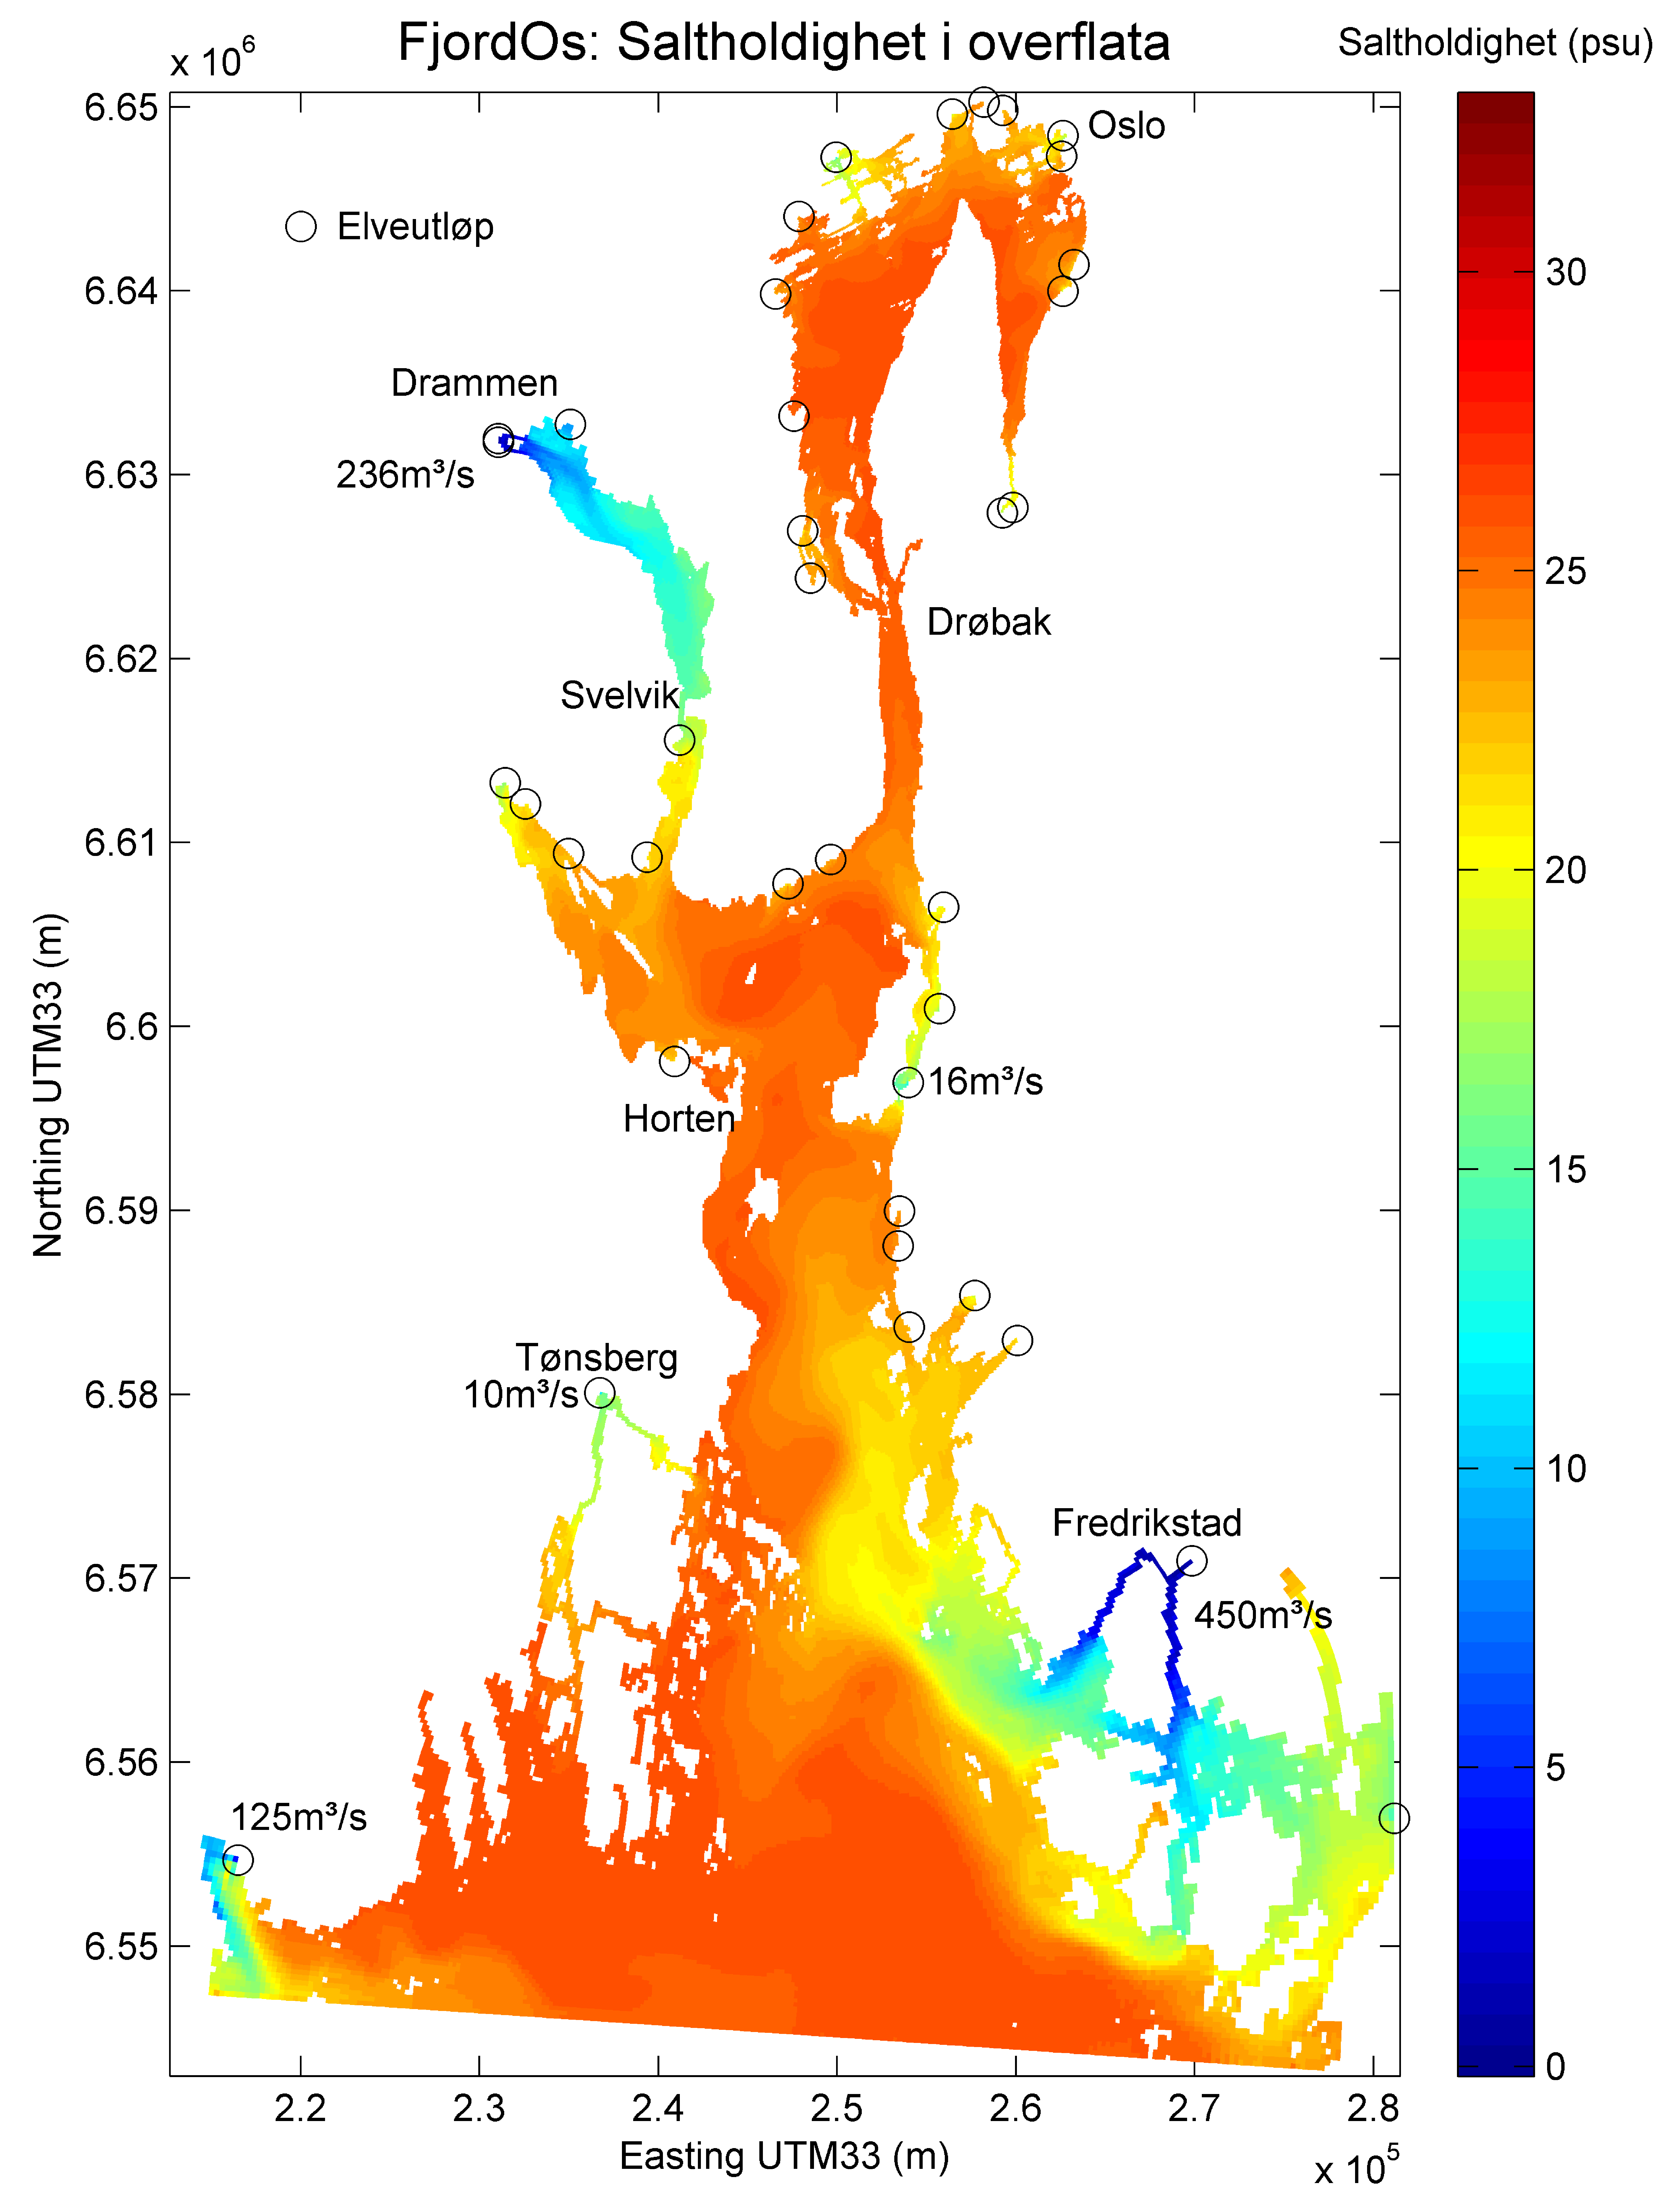
\includegraphics[height=9cm]{fjordos_rivers}}
  \end{pspicture}
% Figure caption is below the figure
  \caption{Left panel shows the many rivers (blue solid lines) emptying freshwater to the fjord (from NVE elvenett). The red numbers indicate a Main Catchment Area (MCA). The red dots indicate the location of the individual rivers discharging freshwater to Oslofjord (cf. Table \ref{tab:rivers01}). Some of the larger rivers, for instance Glomma, Drammenselva and Numedalsl{\aa}gen, are marked with a thicker blue line. Stations with water discharge measurements are shown with green dots and numbered with black numbers, e.g. q8. Right panel shows the location of the 37 rivers named in Table \ref{tab:rivers01}. }   
  \label{fig:rivers01}      
 \end{center}
\end{figure}
%

 

To obtain the necessary information on the freshwater discharges to the Oslofjord within the FjordOs CL model domain we make use of discharge data from a database constructed by use of the hydrological model HBV \citep{beldr:etal:2003}. In essence the HBV model provides an estimate of the daily mean freshwater drained into the ocean (or fjord) from a preselected set of so called Main Catchment Areas (MCAs). Each MCA has in turn at least one or more rivers with an outlet to the sea. Let $Q_i$ be the daily mean freshwater discharged from the $i$th MCA and $A_i$ its area. Furthermore, let $q_{ij}$ be the discharge from the $j$th individual river associated with the $i$th MCA. Then assuming that $q_{ij}$ is entirely determined by the ratio of its local catchment area $a_{ij}$ to the area of the MCA, that is $A_i$ we get
\be
 \label{eq:riv02}
  q_{ij} = \frac{a_{ij}}{A_i} Q_i.
\ee

A total of 15 of Norway's MCAs drains into the Oslofjord within the FjordOs model domain (Figure \ref{fig:rivers01}). These MCAs in turn contain a total of 46 river outlets as listed by Table \ref{tab:rivers01}. Six of these belongs to Glomma and five to Drammenselva. Hence there are 37 named rivers. Their locations are shown by Figure \ref{fig:rivers01}. By use of (\ref{eq:riv02}) and Table \ref{tab:rivers01} we may find the discharge emitted from each of them provided $Q_i$ is known. The HBV database contains information on $Q_i$ from 1962 up to and including the previous year with a lag of about six months. Thus $Q_i$ was not available for 2015 at the time of the simulations presented in this report. Our hindcast period is from April 1, 2014 up to and including December 2015. We must therefore obtain information on $Q_i$ for 2015 from another source. To this end we make use of observations from the NVE website\footnote{\texttt{http://www2.nve.no/h/hd/plotreal/Q/index.html}} available in near real time. If we for instance consider the observed discharge from river $n$ within the $i$th MCA, we find $Q_i$ by rearranging (\ref{eq:riv02}), that is,
\be
 \label{eq:riv03}
  Q_i = A_i\frac{q_{in}}{a_{in}}.
\ee
where $q_{in}$ is the known discharge of the $n$'th river and $a_{in}$ is the size of its local catchment area. Having thus found $Q_i$ we find the discharges from the remaining rivers of that MCA by use of (\ref{eq:riv02}) and the $a_{ij}$'s listed in Table \ref{tab:rivers01}.

Using this method we first calculated the daily mean discharge for MCA numbers $i=1, 2, 3, 6, 8, 12$, and $15$ using the NVE station data for rivers nos. 1 (Iddefjorden/Haldenv.), 2-7 (Glomma), 13 (Mosseelva), 21 (Akerselva), no. 25 (Sandvikselva), 34-38 (Drammenselva) and 46 (Numedalsl{\aa}gen). The NVE station for MCA no. 2 is located far upriver (Figure \ref{fig:rivers01}), so a correction factor is estimated based on a least square fit between the NVE observations at R{\aa}n{\aa}sfoss and the Glommens og Laagens Brukseierforening (glb.no) observations at Sarpfoss for the period up to and including October 28, 2015. The result is
\be
 \label{eq:riv04}
 Q_2 = 1.123 \cdot Q_{\text{R{\aa}n{\aa}sfoss}}.
\ee
This yields an estimate of the river discharge in Glomma with an RMS error of about 100 m$^3$/s. The corresponding discharges, that is, $q_{2j}$ for $j=2,3,\ldots,7$, are found by use of (\ref{eq:riv02}) and the size of the corresponding local catchment areas $a_{2j}$ listed in Table \ref{tab:rivers01}.
%%%%%%%%%%%%%%%%%%%%%%%%%%% Location of rivers %%%%%%%%%%%%%%%%%%%%%%%%%%%%%%%%%%%%%%
\clearpage
\vspace{5mm}
\tablecaption{Rivers in the FjordOs CL model. The outlet positions follow the index convention in ROMS. The position is at a $u$-point if the direction is along the $x$-axis, and at a $v$-point if the direction is along the $y$-axis. The index counting in ROMS starts at 0, except for the $u$-points and $v$-points, where the count starts at 1. MCA: Main Catchment Area.}
\tablefirsthead{\hline 
  River	& MCA	& \mc{1}{c}{Area}	& Outlet	& Outlet	& Direction	& Sign	& Name			\\ 
  No.	& no.   & \mc{1}{c}{$a_{ij}$}	& $x$-pos.	& $y$-pos.	& 0=along $x$	&	&			\\
	&       &			&       	&       	& 1=along $y$	&	&			\\
		\hline }
\tablehead{\hline \mc{8}{l}{\small\slshape continued from previous page}  \\ \hline
  River	& MCA	& \mc{1}{c}{Area}	& Outlet	& Outlet	& Direction	& Sign	& Name			\\ 
  No.	& no.   & \mc{1}{c}{$a_{ij}$}	& $x$-pos.	& $y$-pos.	& 0=along $x$	&	&			\\
	&       &			&       	&       	& 1=along $y$	&	&			\\
		\hline}
\tabletail{\hline \mc{8}{r}{\small\slshape continued on next page}  \\ \hline}
\tablelasttail{\hline}
\begin{center}
% \newcolumntype{d}{D{.}{.}{2}}
 \begin{supertabular}{ccrccccl}
  1	& 1	& 2512.00	& 297		& 44		& 0		& -1	& Iddefjorden/Haldenv.		\\
  2	& 2	& 7222.43	& 261		& 77		& 1		& -1	& Glomma ({\O}sterelva)		\\
  3	& 2	& 7222.43	& 260		& 77		& 1		& -1	& Glomma ({\O}sterelva)		\\
  4	& 2	& 7222.43	& 259		& 77		& 1		& -1	& Glomma ({\O}sterelva)		\\
  5	& 2	& 7222.43	& 258		& 70		& 1		& -1	& Glomma ({\O}sterelva)		\\
  6	& 2	& 7114.64	& 248		& 91		& 0		& -1	& Glomma (Vesterelva)		\\
  7	& 2	& 7114.64	& 248		& 92		& 0		& -1	& Glomma (Vesterelva)		\\
  8	& 3	& 13.90		& 273		& 202		& 0		& -1	& Krokstadbekken		\\
  9	& 3	& 25.90		& 251		& 230		& 1		& -1	& Heiabekken+Kure{\aa}a		\\
  10	& 3	& 7.57		& 213		& 219		& 1		& -1	& St{\o}tvikbekken		\\
  11	& 3	& 3.83		& 211		& 258		& 1		& +1	& Evje{\aa}a			\\
  12	& 3	& 5.55		& 213		& 275		& 1		& -1	& Gunnarbybekken		\\
  13	& 3	& 688.34	& 221		& 337		& 0		& -1	& Mossevassdraget		\\
  14	& 3	& 19.33		& 239		& 373		& 0		& -1	& Kambobekken			\\
  15	& 4	& 138.49	& 242		& 423		& 0		& -1	& H{\ae}lenelva			\\
  16	& 5	& 6.94		& 273		& 634		& 1		& +1	& Gloslibekken			\\
  17	& 5	& 51.72		& 280		& 638		& 1		& +1	& {\AA}rungelva			\\
  18	& 5	& 85.97		& 286		& 784		& 0		& -1	& Gjersj{\o}elva		\\
  19	& 6	& 39.10		& 289		& 802		& 0		& -1	& Ljanselva			\\
  20	& 6	& 69.26		& 267		& 864		& 0		& -1	& Alna				\\
  21	& 6	& 237.81	& 266		& 876		& 1		& -1	& Akerselva                	\\
  22	& 6	& 23.24		& 226		& 890		& 1		& -1	& Frognerbekken            	\\
  23	& 7	& 14.46		& 213		& 895		& 0		& -1	& Hoffelva               	\\
  24	& 7	& 176.30	& 188		& 888		& 1		& -1	& Lysakerelva                	\\
  25	& 8	& 227.72	& 83		& 843		& 1		& -1	& Sandvikselva                 	\\
  26	& 8	& 21.74		& 72		& 782		& 1		& -1	& Neselva			\\
  27	& 9	& 37.63		& 84		& 726		& 1		& +1	& Askerelva                   	\\
  28	& 9	& 2.82		& 126		& 665		& 1		& +1	& N{\ae}rsneselva		\\
  29	& 9	& 112.95	& 149		& 607		& 0		& +1	& {\AA}rosvassdraget		\\
  30	& 9	& 19.05		& 158		& 584		& 0		& +1	& S{\ae}treelva               	\\
  31	& 10	& 18.01		& 179		& 447		& 1		& -1	& Tofteelva			\\
  32	& 10	& 35.47		& 156		& 435		& 1		& -1	& Sageneelva			\\
  33	& 11	& 309.38	& 22		& 621		& 1		& -1	& Lierelva			\\
  34	& 12	& 2139.31	& 1		& 611		& 0		& +1	& Drammeneslva 1		\\
  35	& 12	& 4278.61	& 1		& 610		& 0		& +1	& Drammenselva 2		\\
  36	& 12	& 4278.61	& 1		& 609		& 0		& +1	& Drammenselva 3		\\
  37	& 12	& 4278.61	& 1		& 608		& 0		& +1	& Drammenselva 4		\\
  38	& 12	& 2139.31	& 1		& 607		& 0		& +1	& Drammeneslva 5		\\
  39	& 12	& 8.11		& 97		& 501		& 1		& -1	& Ebbestadelva   		\\
  40	& 12	& 14.54		& 82		& 447		& 0		& +1	& Bergerelva    		\\
  41	& 13	& 6.59		& 42		& 450		& 1		& -1	& Sandobekken    		\\
  42	& 13	& 29.84		& 22		& 472		& 1		& -1	& Selvikelva  			\\
  43	& 13	& 193.23	& 13		& 481		& 1		& -1	& Sandevassdraget   		\\
  44	& 13	& 33.66		& 93		& 351		& 1		& +1	& Borreelva       		\\
  45	& 14	& 1115.00	& 61		& 186		& 0		& +1	& Aulivassdraget      		\\
  46	& 15	& 6514.00	& 9		& 23		& 0		& -1	& Numedalsl{\aa}gen  		\\
 \end{supertabular}
\label{tab:rivers01}
\end{center}
\vspace{5mm}



For some of the 15 MCAs in the model domain, no observations are available ($i=$ 4, 5, 7, 9, 10, 11, 13, 14). We have estimated $Q_i$ for these rivers using the $Q_i$'s from MCA nos. 2 (Glomma), 3 (Mosseelva), 8 (Sandvikselva) and 15 (Nummedalsl{\aa}en). An auxiliary parameter was calculated that was the sum of the river discharges of all combinations of the four rivers. A least mean square fit was performed between this new parameter and the discharge for the MCA in question, namely 
\be
 \label{eq:riv05}
 Q_i = \alpha_i \left(f_{i2} Q_2 + f_{i3} Q_3 + f_{i8} Q_8 +f_{i15} Q_{15}\right) + \beta_i .
\ee
The result of this analysis is shown in Table \ref{tab:rivers04}. It is somewhat surprising that the discharge from MCA nos. 2 and 15 did not influence the estimate of the discharge from the other MCAs.   
%%%%%%%%%%%%%%%%%%%%%%%%%%% Summary of experiments %%%%%%%%%%%%%%%%%%%%%%%%%%%%%%%%%%%%%%
%\clearpage
\begin{table}[t]
 \caption{Estimating discharges in unobserved MCAs based on observations
 at four MCAs with observations using the least mean square fit (\ref{eq:riv05}).}
 \label{tab:rivers04}       % Give a unique label
% For LaTeX tables use
 \centering
% \begin{center}
   \begin{tabular}{ccccccc}
   \hline
   MCA & $f_{i2}$ & $f_{i3}$ & $f_{i8}$ & $f_{i15}$ & $\alpha_i$ & $\beta_i$  \\
   no. &          &          &          &           &            &            \\ 
   \hline
   4   & 0        &  1       &  0       &  0        & 0.201      &  0.120     \\
   5   & 0        &  1       &  0       &  0        & 0.265      &  0.274     \\
   7   & 0        &  0       &  1       &  0        & 0.625      &  0.531     \\
   9   & 0        &  0       &  1       &  0        & 0.750      &  0.209     \\
   10  & 0        &  0.5     &  0.5     &  0        & 0.264      & -0.276     \\
   11  & 0        &  0       &  1       &  0        & 1.317      &  0.417     \\
   13  & 0        &  0       &  1       &  0        & 1.081      &  0.998     \\
   14  & 0        &  0.5     &  0.5     &  0        & 1.000      &  1.087     \\
   \hline
   \end{tabular}
% \end{center}
\end{table}



Finally we emphasize that the rivers, in addition to providing freshwater to the fjord, are sources of nutrients, organic matter, bacteria, particles and contaminants. Several of these parameters are monitored in the national monitoring program \citep[Riverine Inputs and direct Discharges - RID,][]{skarb:etal:2011}. It is therefore possible to include information from the RID program in the river forcing, and hence the FjordOs CL model may be used in the future to model dispersion of any of the RID parameters.







